\subsection{User Interface Design}
When designing an interface, the purpose of the service comes into question. It is important to define what drives each page of the application, and what the core functionality of it is in order to choose the best layout and color scheme for the component\textquotesingle s representation and the user\textquotesingle s accessibility. In addition, identifying the core user base is also important in designing the interface.

\subsubsection{Interface Color Selection}
For this service, some pages are visually driven, with little text on the screen, while some are text driven. The Catalog page for instance relies on the data visualization component as the main focal point, while the settings page contains only text. This presents a bit of a conflict as to which colors to choose for a service wide color palette.\par
With pages that are mainly visually driven, like the Catalog page, it is best to use darker background colors to help the visuals stand out compared to the rest of the page. For text however it is best to use lighter color backgrounds as to not cause strain on the reader\textquotesingle s eyes. Thus it is decided that the service will be mostly light colored backgrounds, with some colored components.\par
For the Catalog page, it is important for the data visualizations to stand out. Contrast in pages is important for drawing attention to elements and directing the user\textquotesingle s eyes. The analysis section of the page should have a background color to make it stand out against the rest of the page.\par
As for the actual color palette selection, our sponsor has a logo made up for his research that contains core colors of yellow and black. We liked this logo from the get go and wanted to incorporate these colors into the application. We aim to follow the 60-30-10 rule using a palette of white yellow and black.

\subsubsection{Page Organization}
Page organization is important for putting elements in a logical and meaningful place. Placing related content together helps the end user be more efficient, especially on pages like the Job Creation page. The following thought process went into each page.\par
The Catalog page contains the user\textquotesingle s results from past jobs, and allows them to filter through them and view the analysis for whichever they\textquotesingle d like. The main component of this page is again the data visualizations, so it is important that this component take up most of the space on the page. The side components, that being the filtering section and the results table, take up a third of the screen and are aligned to the left, while the data visualizations take up the other two thirds and the right side of the screen. This helps to divide up the content for the user, and make filtering and navigating the results table easier.\par
The Settings page acts as a standard panel for global application preferences. This is implemented as a simple form primarily consisting of three components: Account Settings, Group Server Access, and Processing. The Account Settings component allows users to change both their email addresses and passwords associated with their accounts. The Group Server Access component lists information (role, IP address, and login credentials for the server) on each of the remote servers associated with a user\textquotesingle s account and allows them to modify it (with respect to their role). In addition, for each remote server, the component also allows the user to invite new members to the group by providing their email. The Processing component is a simple list of radio buttons to specify which server the user currently wants to process jobs with.\par
The Job Creation page is where users will define and start jobs on their sets of sound files. The organization of this page is based on the step by step process of starting jobs. When a user first visits this page, they will see a group of buttons which are used to select the index that the analysis will use. On loading the page, they will also see a button to change their working directory and a list of wav files contained in the current working directory. A user could either choose an index or specify the files they would like to analyze as the first action. Once the index and files have been specified, the stepper component will move to the next step and the parameter specification components will become visible. The use of a Stepper component will make sure the user is clear on all steps that need to be taken to successfully start a job. When all required information has been inputted, the user will be free to start the job. After starting the job, the user will be notified that it started successfully and will be given the option to navigate to the In Progress Jobs page, to view the state of jobs not yet completed. If the user would like to start a new job, the set of files previously analyized will remain selected for ease of use, as it is common to run multiple indices on the same files.\par

\subsubsection{Page Use Cases}
\begin{center}
  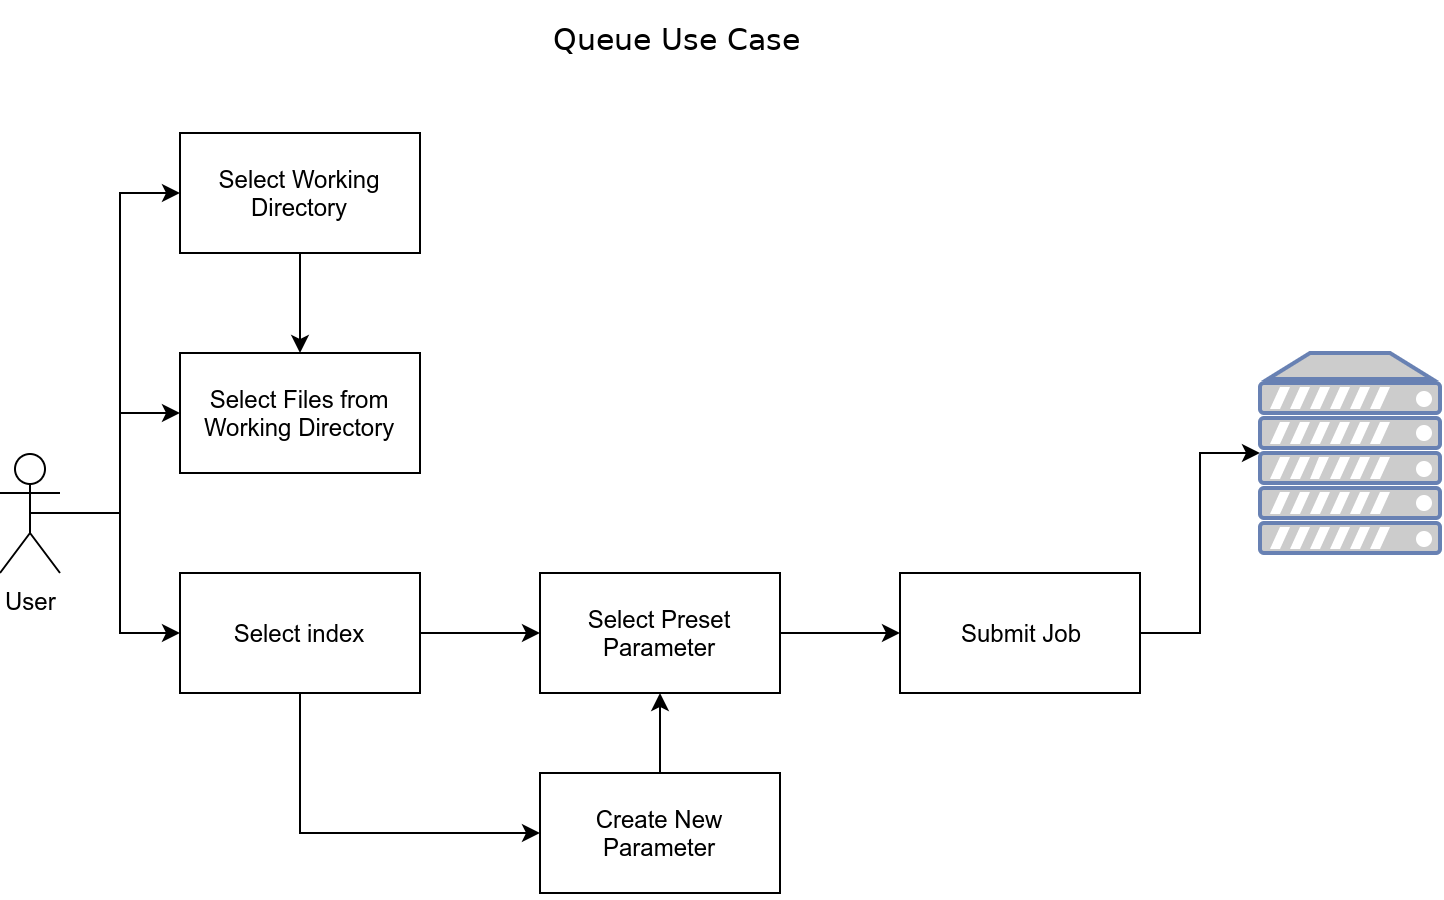
\includegraphics[width=\textwidth]{UsecaseQueue} \\[12pt]
\end{center}
\begin{center}
  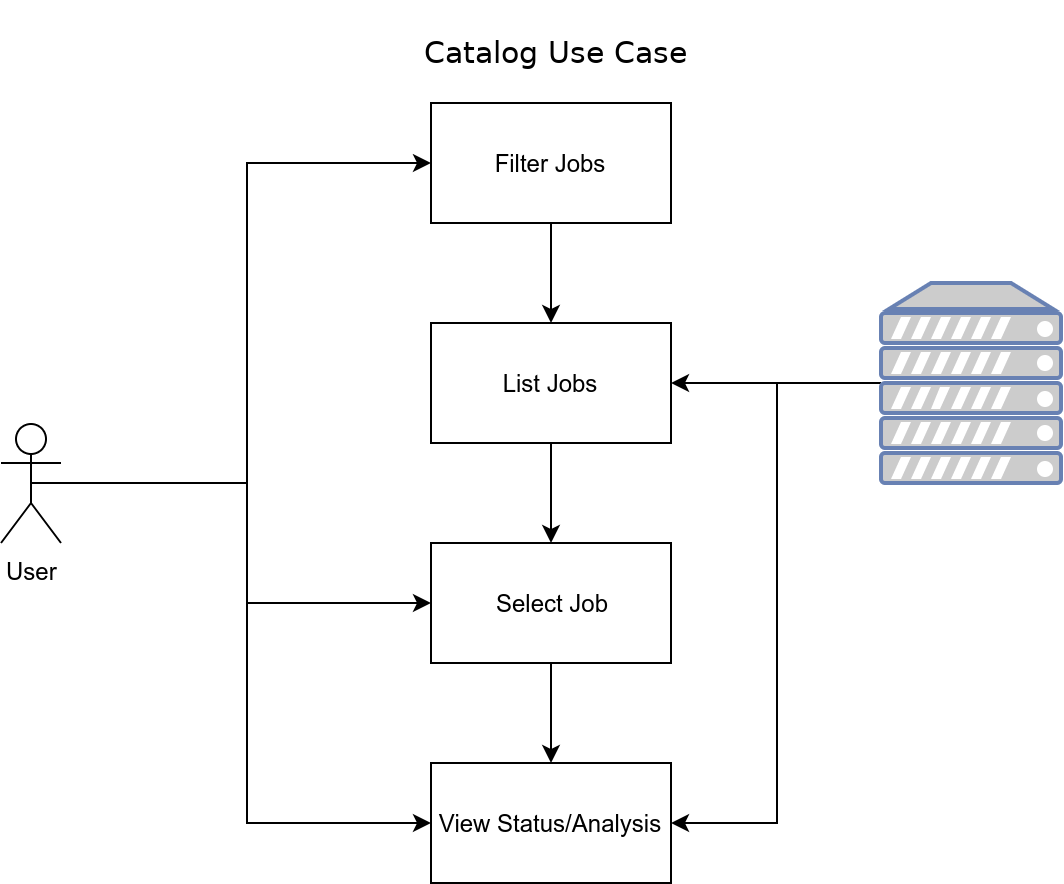
\includegraphics[width=0.85\textwidth]{UsecaseCatalog} \\[12pt]
\end{center}
\begin{center}
  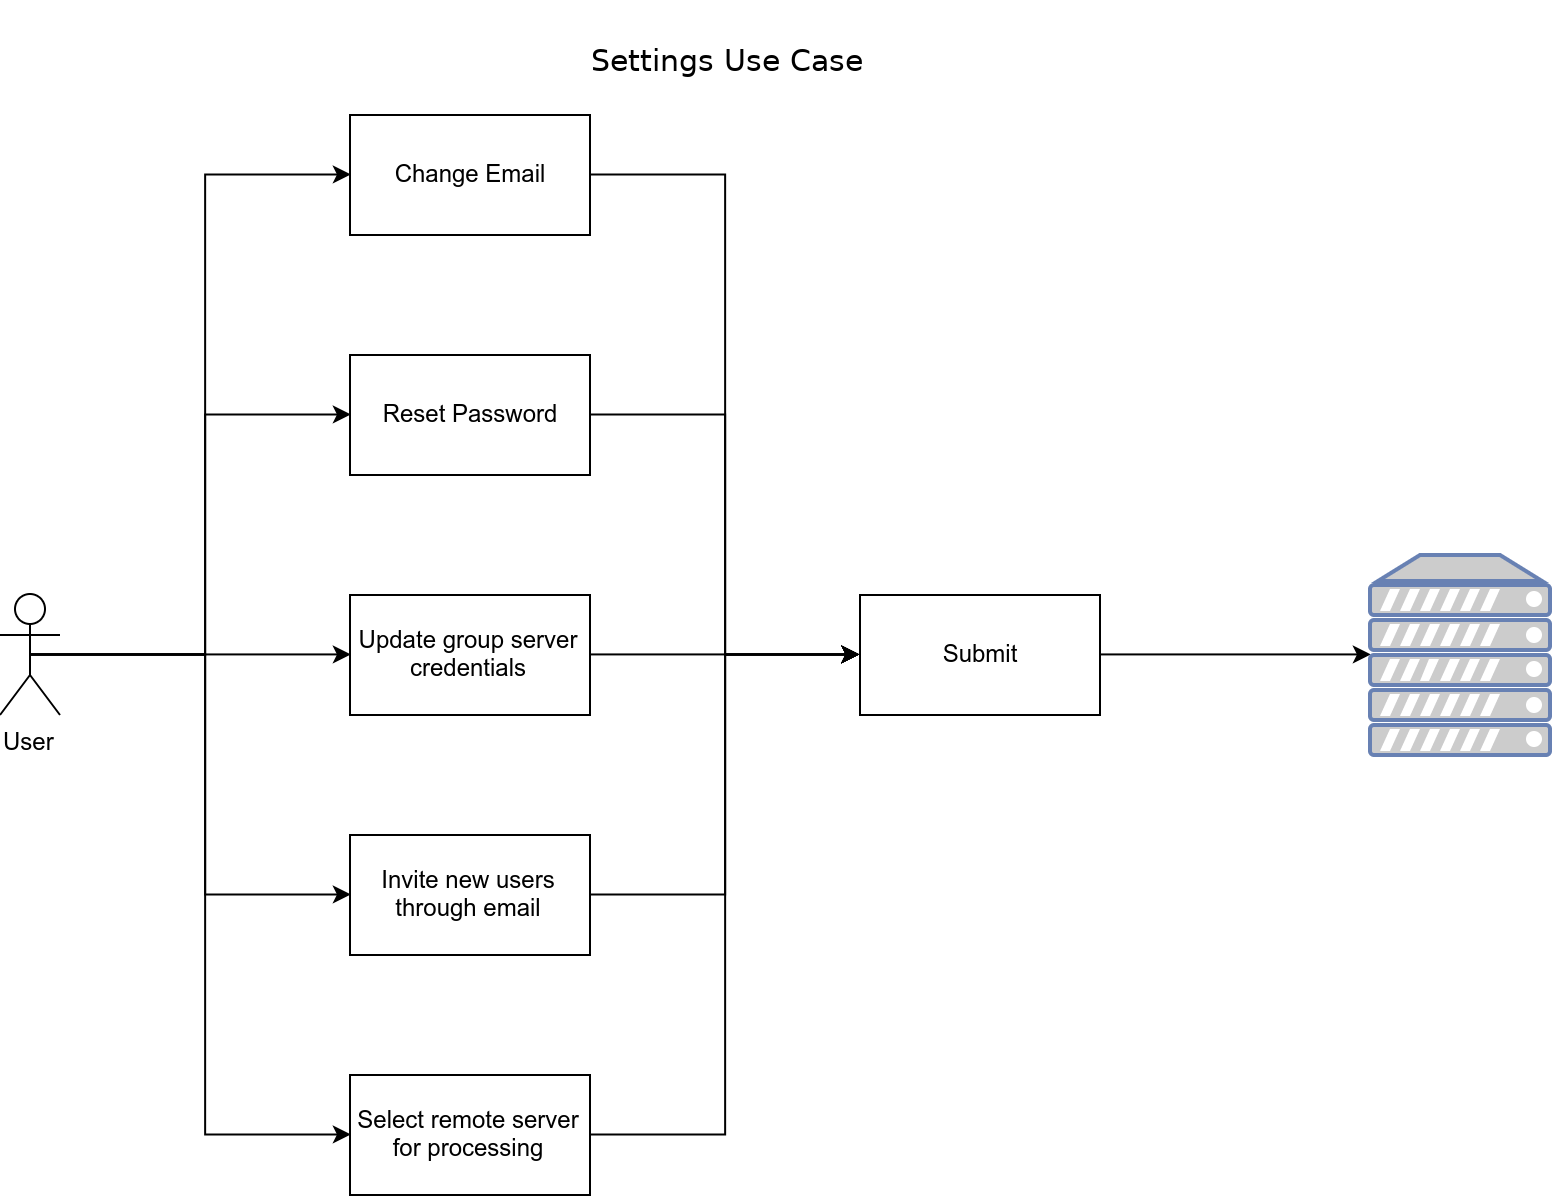
\includegraphics[width=\textwidth]{UsecaseSettings} \\[12pt]
\end{center}

\subsubsection{Frontend Frameworks}
A big part of getting the front end of the service up and running as quickly as we did was the use of frameworks. The core frameworks for this project are explained in the Infrastructure section of this project, so this will only cover the core frontend frameworks. The core frameworks used are as follows:
\begin{itemize}
  \item Material-UI
  \item Bootstrap
  \item Recharts
\end{itemize}
Material-UI is a framework for React that includes new components to easily add into the existing pages, handling styling for these components to help save time in development. This framework is used heavily in both the Catalog and Job Creation pages.\par
Bootstrap is a CSS framework made to handle screen size changes without hassle on the developer\textquotesingle s end. Bootstrap divides the page up into twelve parts, containing rows and columns. Components can then be placed into their respective rows and columns, including nesting, to create a functional and dynamic interface. This framework is especially useful for us to handle changing screen sizes.\par
For the analysis part of the Catalog page, we needed a framework to turn our JSON data into graphics based on the user selected result from the result table. Recharts is a framework for doing just that, and is in charge of creating the respective data visualizations for each index. Recharts provides easy to use code made specifically for React to turn our data into nice, concise graphics.
